\documentclass[dvipsnames]{beamer}
\input{mybeamerdefs}

\begin{document}

\begin{frame}{\today}
\begin{itemize}
\item I wrote a script to show that we can simulate the ems in parallel and do the reconstruction afterwards.
\end{itemize}
\end{frame}

\section{Simulating ems in parallel}

\begin{frame}{Summary}
\begin{itemize}
\item I simulated 2DFT+reconstruction with four ems using the script of 2019-12-11.
\item I ran the same simulation with two of the four ems and stored the MR signals. I repeated the simulation with the other two ems and stored the MR signals. I summed the MR signals and did the reconstruction.
\end{itemize}
\end{frame}

\begin{frame}{4 ems in one run}
\begin{center}
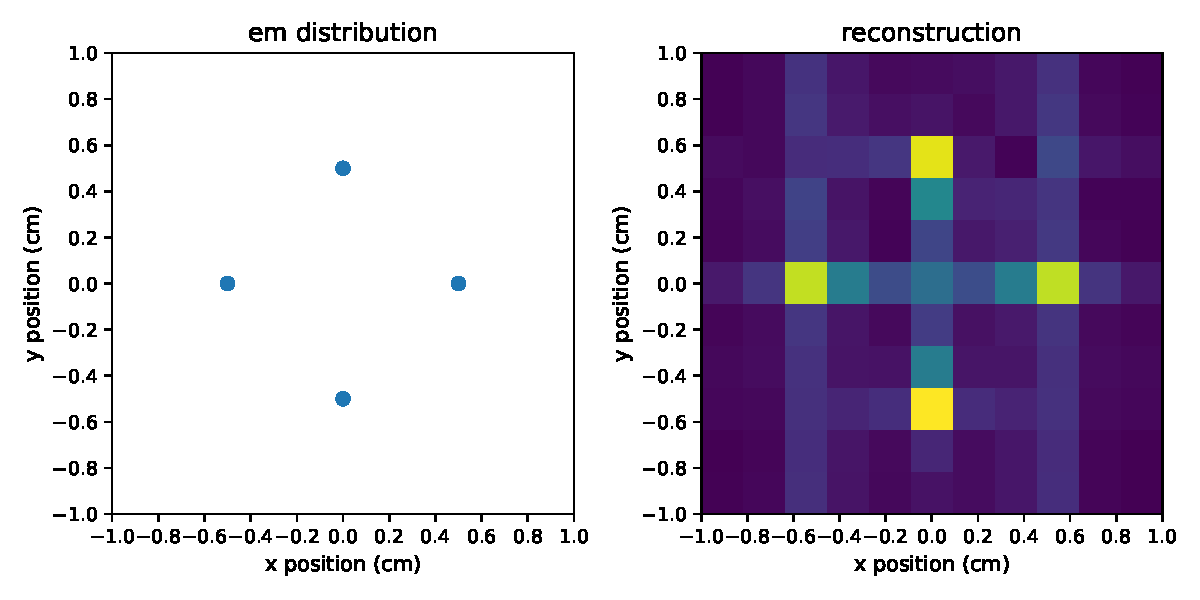
\includegraphics[width=\textwidth]{reconstruction_single}
\end{center}
\end{frame}

\begin{frame}{2 ems in run 1, 2 ems in run 2}
\begin{center}
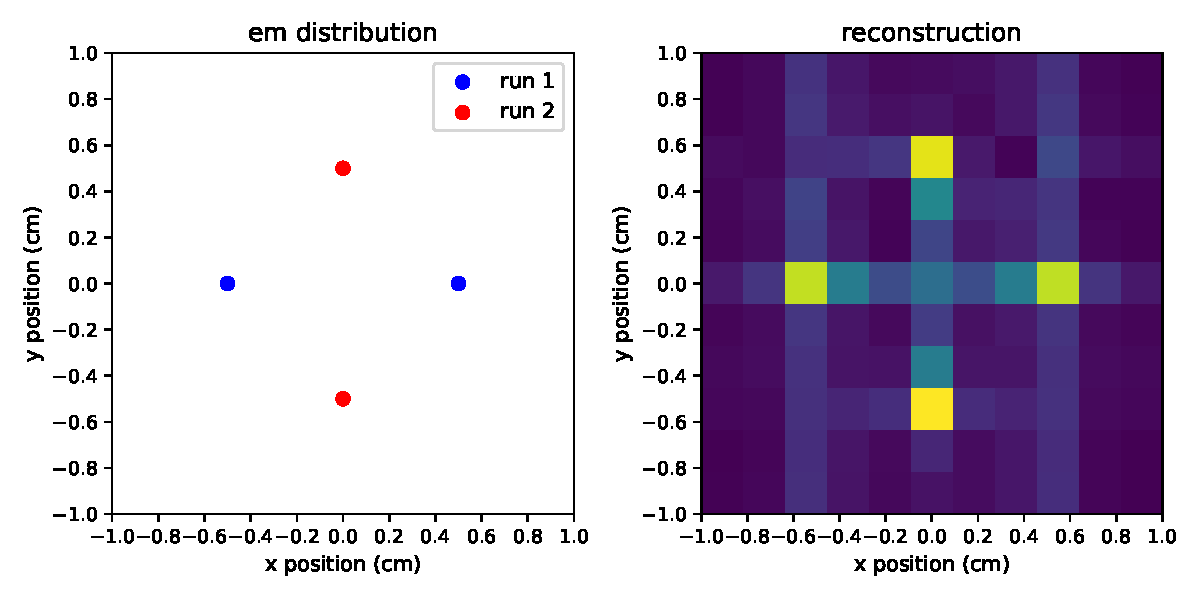
\includegraphics[width=\textwidth]{reconstruction_parallel}
\end{center}
\end{frame}

\begin{frame}{Comments}
\begin{itemize}
\item The reconstructions are identical.
\item We can parallelize the simulation easily. A central computer partitions the ems across the cluster. Each computer simulates its own set of ems and stores the MR signals. Once the simulation is complete, each computer sends the MR signals to the central computer. The central computer does the reconstruction.
\end{itemize}
\end{frame}

\end{document}